\documentclass[11pt,a4paper]{article}
\usepackage{fontspec}
\usepackage[polish]{babel}
\usepackage[margin=2.2cm]{geometry}
\usepackage{graphicx}
\usepackage[table]{xcolor}
\usepackage{listings}
\usepackage{tikz}
\usepackage{amsmath}
\usepackage{booktabs}
\usepackage{caption}
\usepackage{float}
\usepackage{enumitem}
\usepackage{fancyhdr}
\usepackage[hidelinks]{hyperref}

\definecolor{pwr}{HTML}{A4161A}
\definecolor{kod}{HTML}{F6F6F6}

\lstset{
  language=VHDL,
  basicstyle=\ttfamily\small,
  keywordstyle=\color{pwr}\bfseries,
  commentstyle=\color{gray}\itshape,
  backgroundcolor=\color{kod},
  frame=single, rulecolor=\color{gray!40},
  numbers=left, numberstyle=\tiny\color{gray},
  breaklines=true, columns=fullflexible, keepspaces=true,
  xleftmargin=1.5em, framexleftmargin=1.5em
}

\captionsetup{font=small,labelfont=bf}
\setlength{\parindent}{0pt}
\setlength{\parskip}{0.6em}
\setlength{\headheight}{14pt}

\pagestyle{fancy}
\fancyhf{}
\lhead{\small UCiSW 1, laboratorium 1}
\rhead{\small Korwin, Kasiarz}
\cfoot{\thepage}

\newcommand{\nx}[1]{\overline{x}_{#1}}
\newcommand{\jj}{\cellcolor{pwr!18}1}

% mapa Karnaugha: wiersze x3x2 = 00, 01, 11, 10; kolumny x1x0 = 00, 01, 11, 10
\newcommand{\kmap}[5]{%
  \begin{tabular}{c|cccc}
    \multicolumn{5}{c}{\textbf{#1}}\\[2pt]
    $x_3x_2 \backslash x_1x_0$ & 00 & 01 & 11 & 10\\ \hline
    00 & #2\\
    01 & #3\\
    11 & #4\\
    10 & #5
  \end{tabular}}

\begin{document}

% ---------------- strona tytulowa ----------------
\begin{titlepage}
\centering

\includegraphics[width=3.2cm]{img/pwr_logo.png}\par\vspace{0.8cm}
{\Large\bfseries Politechnika Wrocławska}\par\vspace{2.5cm}
{\large Układy Cyfrowe i Systemy Wbudowane 1}\par\vspace{0.3cm}
{\large Laboratorium}\par\vspace{1.2cm}
{\color{pwr}\rule{0.6\textwidth}{0.8pt}}\par\vspace{0.5cm}
{\LARGE\bfseries Sprawozdanie z laboratorium 1}\par\vspace{0.4cm}
{\Large Czterobitowy układ kombinacyjny}\par\vspace{0.2cm}
{\large wariant c): $Y = (4 - X) \bmod 16$}\par\vspace{0.5cm}
{\color{pwr}\rule{0.6\textwidth}{0.8pt}}\par
\vfill
\begin{tabular}{ll}
\textbf{Wykonali:} & Adam Korwin, 284455\\
                   & Dawid Kasiarz, 284541\\[6pt]
\textbf{Prowadzący:} & dr inż. Jarosław Sugier\\[6pt]
\textbf{Data zajęć:} & 20.10.2026
\end{tabular}
\vspace{1.5cm}
\end{titlepage}

% ---------------- tresc ----------------
\section{Treść zadania}

Celem ćwiczenia było zaprojektowanie czterobitowego układu kombinacyjnego, który dla wejścia $X$ wyznacza wartość $Y = (4 - X) \bmod 16$. Oba wektory, \texttt{X(3 downto 0)} oraz \texttt{Y(3 downto 0)}, są zapisane w naturalnym kodzie binarnym (NKB). Ćwiczenie składało się z czterech zadań:

\begin{description}[leftmargin=2.2em,style=sameline]
  \item[Z1] minimalizacja funkcji $Y(0)$ do $Y(3)$ w tablicach Karnaugha, opis układu w VHDL i symulacja behawioralna dla wszystkich wartości $X$ od 0 do 15, zmienianych co 100~ns;
  \item[Z2] uruchomienie układu na płycie, gdzie $X$ pochodzi z przełączników \texttt{PL\_USER\_SW(3:0)}, a $Y$ steruje diodami \texttt{PL\_USER\_LED(3:0)}, oraz symulacja czasowa przełączania bitów $Y$ przy zmianie $Y\colon 8 \to 7$;
  \item[Z3] diagram blokowy, w którym układ z Z1 jest osobnym modułem, a wartości $X$ i $Y$ są pokazywane na wyświetlaczu OLED (\texttt{OLED\_1x32});
  \item[Z4] realizacja tego samego działania przy pomocy gotowego bloku IP \emph{Adder/Subtracter} i porównanie obu wyników na wyświetlaczu.
\end{description}

\section{Z1: projekt układu i symulacja behawioralna}

\subsection{Tablica prawdy}

Dla $X \le 4$ wynik jest po prostu różnicą $4 - X$. Dla $X \ge 5$ różnica jest ujemna, więc do wyniku dodajemy 16. Pełną tablicę zawiera tabela~\ref{tab:prawda}.

\begin{table}[H]
\centering
\small
\begin{tabular}{rcrc@{\hspace{2.5em}}rcrc}
\toprule
$X$ & $x_3x_2x_1x_0$ & $Y$ & $y_3y_2y_1y_0$ & $X$ & $x_3x_2x_1x_0$ & $Y$ & $y_3y_2y_1y_0$\\
\midrule
0 & 0000 & 4  & 0100 & 8  & 1000 & 12 & 1100\\
1 & 0001 & 3  & 0011 & 9  & 1001 & 11 & 1011\\
2 & 0010 & 2  & 0010 & 10 & 1010 & 10 & 1010\\
3 & 0011 & 1  & 0001 & 11 & 1011 & 9  & 1001\\
4 & 0100 & 0  & 0000 & \textbf{12} & \textbf{1100} & \textbf{8} & \textbf{1000}\\
5 & 0101 & 15 & 1111 & \textbf{13} & \textbf{1101} & \textbf{7} & \textbf{0111}\\
6 & 0110 & 14 & 1110 & 14 & 1110 & 6  & 0110\\
7 & 0111 & 13 & 1101 & 15 & 1111 & 5  & 0101\\
\bottomrule
\end{tabular}
\caption{Tablica prawdy układu. Pogrubione wiersze odpowiadają zmianie $Y\colon 8 \to 7$ badanej w zadaniu Z2.}
\label{tab:prawda}
\end{table}

\subsection{Minimalizacja w tablicach Karnaugha}

W mapach wiersze opisują $x_3x_2$, a kolumny $x_1x_0$, obie osie w kodzie Graya. Pola z jedynkami są wyróżnione kolorem.

\begin{figure}[H]
\centering
\small
\kmap{$Y(3)$}{0&0&0&0}{0&\jj&\jj&\jj}{\jj&0&0&0}{\jj&\jj&\jj&\jj}
\hspace{2em}
\kmap{$Y(2)$}{\jj&0&0&0}{0&\jj&\jj&\jj}{0&\jj&\jj&\jj}{\jj&0&0&0}
\\[1.2em]
\kmap{$Y(1)$}{0&\jj&0&\jj}{0&\jj&0&\jj}{0&\jj&0&\jj}{0&\jj&0&\jj}
\hspace{2em}
\kmap{$Y(0)$}{0&\jj&\jj&0}{0&\jj&\jj&0}{0&\jj&\jj&0}{0&\jj&\jj&0}
\caption{Tablice Karnaugha dla bitów wyniku.}
\end{figure}

Odczytane grupy:

\textbf{$Y(0)$.} Jedynki zajmują dwie środkowe kolumny, czyli wszystkie pola z $x_0 = 1$. Bit najmłodszy jest więc kopią wejścia. Wynika to z tego, że odejmowanie od liczby parzystej nie zmienia parzystości.

\textbf{$Y(1)$.} Jedynki leżą w kolumnach 01 i 10, które nie są ze sobą sąsiednie. Powstają dwie grupy po osiem pól, $x_1\nx{0}$ oraz $\nx{1}x_0$, czyli funkcja XOR.

\textbf{$Y(2)$.} Grupa $x_2x_1$ obejmuje wiersze 01 i 11 w kolumnach 11 i 10. Grupa $x_2x_0$ obejmuje te same wiersze w kolumnach 01 i 11. Ostatnia grupa, $\nx{2}\nx{1}\nx{0}$, łączy pola $X = 0$ oraz $X = 8$, bo skrajne wiersze mapy są sąsiednie.

\textbf{$Y(3)$.} Cały wiersz 10 daje $x_3\nx{2}$. Pola $X = 8$ i $X = 12$ w kolumnie 00 dają $x_3\nx{1}\nx{0}$. W wierszu 01 pozostają pola $X = 5, 6, 7$, które pokrywamy grupami $\nx{3}x_2x_1$ oraz $\nx{3}x_2x_0$.

Otrzymane równania:
\begin{align*}
Y(0) &= x_0\\
Y(1) &= x_1\nx{0} + \nx{1}x_0 = x_1 \oplus x_0\\
Y(2) &= x_2x_1 + x_2x_0 + \nx{2}\nx{1}\nx{0} = \overline{x_2 \oplus (x_1 + x_0)}\\
Y(3) &= x_3\nx{2} + x_3\nx{1}\nx{0} + \nx{3}x_2x_1 + \nx{3}x_2x_0
\end{align*}

Poprawność równań sprawdziliśmy dodatkowo krótkim skryptem w Pythonie, który porównuje wynik równań z wartością $(4 - X) \bmod 16$ dla wszystkich szesnastu wartości $X$.

\subsection{Opis w VHDL}

Równania zapisaliśmy bezpośrednio jako przypisania współbieżne w encji \texttt{Z1}. Przy mieszaniu operatorów \texttt{and} i \texttt{or} każdy iloczyn jest ujęty w nawiasy, ponieważ VHDL nie nadaje tym operatorom różnych priorytetów.

\lstinputlisting[caption={Plik \texttt{Z1\_c.vhd}}]{../Z1_c.vhd}

\begin{figure}[H]
\centering
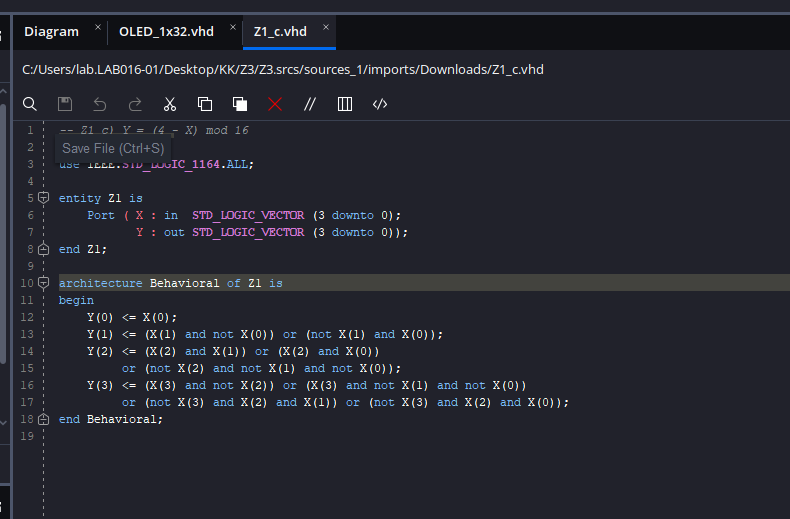
\includegraphics[width=0.75\textwidth]{img/z1_vivado.png}
\caption{Plik \texttt{Z1\_c.vhd} otwarty w edytorze Vivado na zajęciach.}
\end{figure}

\subsection{Testbench i wynik symulacji}

Testbench podaje na wejście kolejne wartości $X$ co 100~ns, dokładnie w sposób podany w poleceniu (\texttt{X <= "0000", "0001" after 100 ns, ...}). Dodaliśmy do niego proces \texttt{Check}, który w połowie każdego kroku porównuje $Y$ z wartością oczekiwaną i w razie niezgodności wypisuje komunikat \texttt{Blad dla X = ...}.

\lstinputlisting[caption={Plik \texttt{Z1\_tb.vhd}}]{../Z1_tb.vhd}

Symulacja zakończyła się komunikatem \texttt{Koniec testu} w chwili 1600~ns i nie pojawił się żaden komunikat o błędzie. Przebiegi z symulacji pokazuje rysunek~\ref{fig:beh}.

\begin{figure}[H]
\centering
\begin{tikzpicture}[x=0.92cm,y=1cm,font=\footnotesize]
  \fill[pwr!12] (13,-0.4) rectangle (14,1.4);
  \node[anchor=east] at (-0.1,1) {\texttt{X}};
  \node[anchor=east] at (-0.1,0) {\texttt{Y}};
  \foreach \i/\y in {0/4,1/3,2/2,3/1,4/0,5/F,6/E,7/D,8/C,9/B,10/A,11/9,12/8,13/7,14/6,15/5} {
    \foreach \v/\lab in {1/\i,0/\y} {
      \draw (\i,\v) -- (\i+0.08,\v+0.25) -- (\i+0.92,\v+0.25) -- (\i+1,\v)
            -- (\i+0.92,\v-0.25) -- (\i+0.08,\v-0.25) -- cycle;
      \node at (\i+0.5,\v) {\lab};
    }
  }
  \draw[gray] (0,-0.6) -- (16,-0.6);
  \foreach \t in {0,2,...,16} {
    \draw[gray] (\t,-0.6) -- (\t,-0.7);
    \pgfmathtruncatemacro{\ns}{\t*100}
    \node[gray,below] at (\t,-0.7) {\ns};
  }
\end{tikzpicture}
\caption{Symulacja behawioralna: $X$ dziesiętnie, $Y$ szesnastkowo, oś czasu w ns. Zaznaczony przedział od 1300~ns to $X = 13$, $Y = 7$.}
\label{fig:beh}
\end{figure}

\section{Z2: uruchomienie na płycie i symulacja czasowa}

\subsection{Przypisanie wyprowadzeń}

Do projektu z Z1 dodaliśmy plik ograniczeń, w którym porty \texttt{X} i \texttt{Y} są przypisane do przełączników SW0 do SW3 i diod LD0 do LD3. Numery wyprowadzeń przepisaliśmy z pliku \texttt{ZU3.xdc} udostępnionego przez prowadzącego. Wszystkie te linie pracują w standardzie \texttt{LVCMOS12}.

\lstinputlisting[language={},caption={Plik \texttt{Z2.xdc}}]{../Z2.xdc}

Po syntezie, implementacji i wygenerowaniu pliku \texttt{.bit} zaprogramowaliśmy układ przez Hardware Manager. Działanie sprawdziliśmy, ustawiając na przełącznikach różne wartości $X$ i porównując stan diod z tabelą~\ref{tab:prawda}.

\subsection{Symulacja czasowa dla zmiany \texorpdfstring{$Y\colon 8 \to 7$}{Y: 8 na 7}}

Wartość $Y = 8$ odpowiada $X = 12$, a $Y = 7$ odpowiada $X = 13$. W testbenchu ta zmiana następuje w chwili 1300~ns. Na wejściu zmienia się tylko jeden bit ($x_0\colon 0 \to 1$), natomiast na wyjściu zmieniają się wszystkie cztery ($1000 \to 0111$). Domyślny czas symulacji w Vivado wynosi 1000~ns, więc w konsoli Tcl wydaliśmy dodatkowo polecenie \texttt{run 500 ns}. Symulację uruchomiliśmy w trybie \emph{Post-Implementation Timing Simulation}, w którym uwzględnione są opóźnienia bramek i połączeń po rozmieszczeniu układu w FPGA.

\begin{figure}[H]
\centering
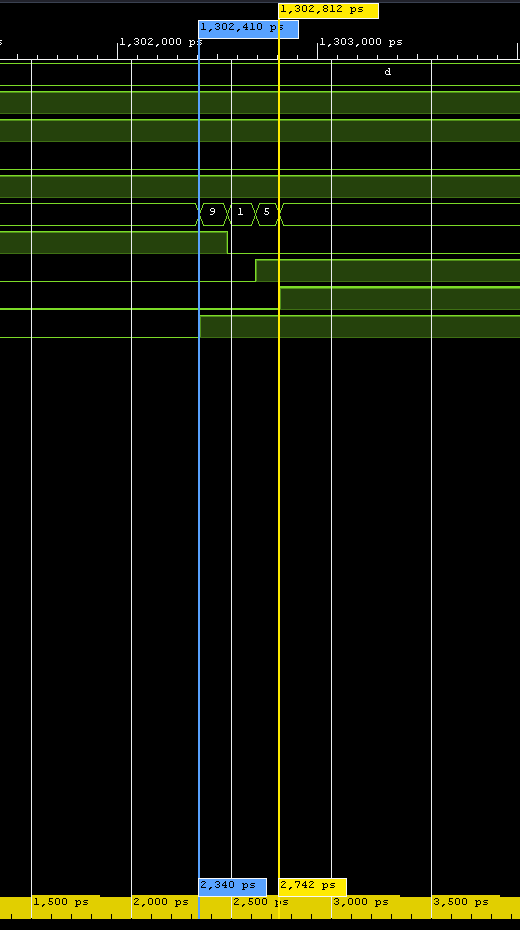
\includegraphics[height=0.5\textheight]{img/timing.png}
\caption{Symulacja czasowa w okolicy 1302~ns. Górny wiersz to szyna $X$ (wartość \texttt{d}), niżej szyna $Y$ z wartościami przejściowymi, a pod nią bity $Y(3)$, $Y(2)$, $Y(1)$, $Y(0)$. Kursory: 1\,302\,410~ps i 1\,302\,812~ps.}
\label{fig:timing}
\end{figure}

Na rysunku~\ref{fig:timing} widać, że bity wyjścia nie zmieniają się jednocześnie. Kolejność zmian odczytana z przebiegu jest zebrana w tabeli~\ref{tab:hazard}.

\begin{table}[H]
\centering
\small
\begin{tabular}{rlcc}
\toprule
czas [ps] & zmieniający się bit & $y_3y_2y_1y_0$ & $Y$\\
\midrule
do 1\,302\,410   & stan początkowy        & 1000 & 8\\
1\,302\,410      & $Y(0)\colon 0 \to 1$   & 1001 & 9\\
ok. 1\,302\,555  & $Y(3)\colon 1 \to 0$   & 0001 & 1\\
ok. 1\,302\,695  & $Y(2)\colon 0 \to 1$   & 0101 & 5\\
1\,302\,812      & $Y(1)\colon 0 \to 1$   & 0111 & 7\\
\bottomrule
\end{tabular}
\caption{Kolejność przełączania bitów wyjścia. Czasy środkowych zmian są odczytane z podziałki z dokładnością kilkunastu pikosekund.}
\label{tab:hazard}
\end{table}

Pierwsza zmiana na wyjściu pojawia się około 2,4~ns po zmianie wejścia. Ten czas obejmuje przejście przez bufor wejściowy, połączenia wewnątrz FPGA i bufor wyjściowy. Najszybciej reaguje $Y(0)$, bo jest to zwykłe połączenie wejścia $x_0$ z wyjściem i sygnał nie przechodzi przez żadną tablicę LUT. Pozostałe bity są liczone w tablicach LUT, a ich ścieżki mają różną długość, dlatego przełączają się później i w różnych chwilach.

W efekcie przez około 400~ps na wyjściu pojawiają się kolejno wartości 9, 1 i 5, których nie ma w tablicy prawdy dla żadnego z dwóch stanów wejścia. Jest to hazard wynikający z różnych opóźnień ścieżek. Każdy pojedynczy bit zmienia się w tym przypadku tylko raz, więc na żadnej linii nie widać krótkiej szpilki, błędny jest dopiero cały wektor. Na diodach takie zjawisko jest niewidoczne, ale gdyby $Y$ był wejściem dla układu synchronicznego, trzeba by próbkować go dopiero po ustaleniu się wszystkich bitów, czyli z okresem zegara dłuższym niż najdłuższe opóźnienie ścieżki.

\section{Z3: diagram blokowy z wyświetlaczem OLED}

W nowym projekcie utworzyliśmy diagram blokowy (\emph{IP Integrator}). Plik \texttt{Z1\_c.vhd} dodaliśmy do diagramu jako moduł RTL (\texttt{Z1\_0}), a obok umieściliśmy moduł \texttt{OLED\_1x32} od prowadzącego. Wyświetlacz pokazuje osiem cyfr szesnastkowych przekazanych przez 32-bitowe wejście \texttt{Line}. Wejście \texttt{Blank} określa, które cyfry są ukryte (jedynka ukrywa cyfrę).

Wejście \texttt{Line} złożyliśmy blokiem \emph{Inline Concat}. Na najmłodsze bity (prawa cyfra wyświetlacza) trafił wynik $Y$, na najstarsze (lewa cyfra) wejście $X$ z przełączników, a pozostałe bity wypełniła stała zero. Wartość \texttt{Blank} = 126 (\texttt{01111110}) ukrywa sześć środkowych cyfr, więc na wyświetlaczu widać układ \texttt{X~~~~~~Y}.

Moduł OLED potrzebuje zegara 100~MHz. Dostarcza go blok \emph{Clocking Wizard} podłączony do różnicowego zegara płyty (\emph{Board}, \emph{Differential Clock}, \emph{Auto Connect}). Z tego powodu w pliku XDC nie ma linii opisujących zegar. Wyjście \texttt{I2C\_NACK} wyprowadziliśmy na diodę LD7, która świeci przy błędzie komunikacji z wyświetlaczem. Porty utworzone poleceniem \emph{Make External} otrzymują przyrostek \texttt{\_0}, więc zmieniliśmy ich nazwy tak, by zgadzały się z plikiem XDC.

\lstinputlisting[language={},caption={Plik \texttt{Z3\_Z4.xdc} (wspólny dla Z3 i Z4)}]{../Z3_Z4.xdc}

\section{Z4: realizacja blokiem Adder/Subtracter}

Do diagramu z Z3 dodaliśmy blok IP \emph{Adder/Subtracter} (\texttt{c\_addsub\_0}) z ustawieniami podanymi w tabeli~\ref{tab:addsub}.

\begin{table}[H]
\centering
\small
\begin{tabular}{ll}
\toprule
parametr & wartość\\
\midrule
Implement using & Fabric\\
Add mode & Subtract\\
Input type, szerokość A i B & Unsigned, 4 bity\\
Output width & 4 bity\\
Latency & 0 (układ czysto kombinacyjny)\\
Clock Enable (zakładka Control) & wyłączone\\
\bottomrule
\end{tabular}
\caption{Konfiguracja bloku \texttt{c\_addsub\_0}.}
\label{tab:addsub}
\end{table}

Na wejście A podaliśmy stałą 4 (\texttt{ilconstant\_2}), a na wejście B wektor $X$ z przełączników. Wyjście bloku ma tylko 4 bity, więc pożyczka z najstarszej pozycji jest odrzucana i wynik odejmowania jest automatycznie liczony modulo 16. Opóźnienie ustawiliśmy na zero, żeby blok nie wymagał zegara i zachowywał się tak samo jak moduł \texttt{Z1}.

Wynik \texttt{S} dołączyliśmy do bloku Concat jako dodatkową cyfrę. Kolejność wejść: \texttt{In0} = $S$ (4 bity), \texttt{In1} = $Y$ (4 bity), \texttt{In2} = stała 0 (20 bitów), \texttt{In3} = $X$ (4 bity). Wartość \texttt{Blank} zmieniliśmy na 124 (\texttt{01111100}), dzięki czemu widoczne są trzy cyfry i wyświetlacz pokazuje \texttt{X~~~~~YS}. Gotowy diagram przedstawia rysunek~\ref{fig:bd}.

\begin{figure}[H]
\centering
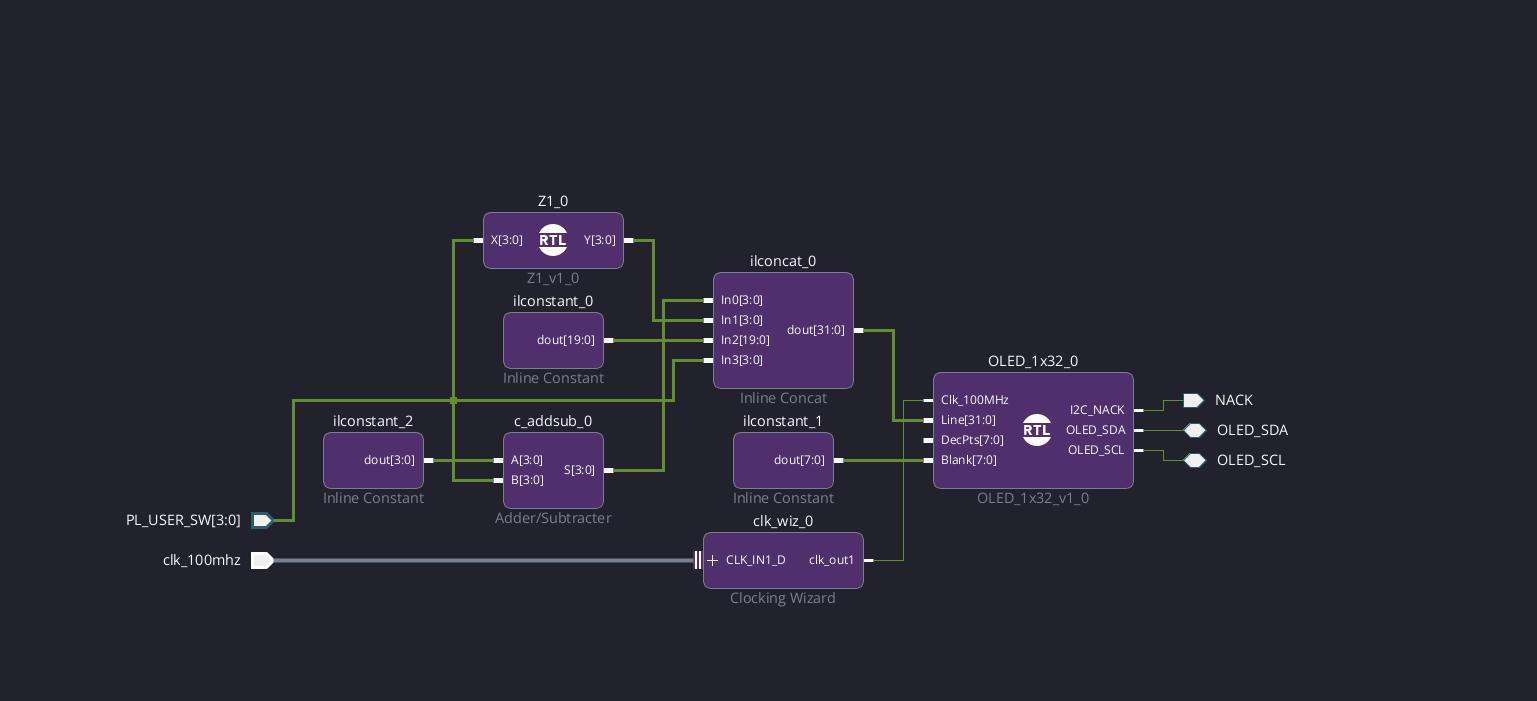
\includegraphics[width=\textwidth]{img/bd.png}
\caption{Diagram blokowy z zadania Z4. Moduł \texttt{Z1\_0} i subtraktor \texttt{c\_addsub\_0} liczą ten sam wynik, a \texttt{OLED\_1x32\_0} wyświetla $X$, $Y$ oraz $S$.}
\label{fig:bd}
\end{figure}

Dla każdego ustawienia przełączników dwie prawe cyfry na wyświetlaczu były takie same, czyli moduł zaprojektowany ręcznie i blok IP dają identyczny wynik.

\section{Wnioski}

Minimalizacja w tablicach Karnaugha dała proste równania. Najmłodszy bit wyniku okazał się zwykłym przewodem, a drugi bit funkcją XOR, co dobrze widać na mapach. Symulacja behawioralna potwierdziła poprawność układu dla wszystkich szesnastu wartości wejścia.

Symulacja czasowa pokazała, że nawet przy zmianie jednego bitu na wejściu wyjście nie przechodzi od razu do nowej wartości. Przy zmianie $Y$ z 8 na 7 przez około 400~ps pojawiały się wartości pośrednie 9, 1 i 5. W układzie sterującym diodami nie ma to znaczenia, ale przy dalszym przetwarzaniu wyniku przez logikę synchroniczną trzeba uwzględnić czas ustalania się wyjścia.

Gotowy blok \emph{Adder/Subtracter} pozwolił uzyskać ten sam wynik bez ręcznej minimalizacji. Przy tak małym układzie obie metody prowadzą do podobnej realizacji w tablicach LUT, natomiast blok IP jest wygodniejszy przy większej liczbie bitów lub innej stałej.

\end{document}
